\documentclass[1p]{elsarticle_modified}
%\bibliographystyle{elsarticle-num}

%\usepackage[colorlinks]{hyperref}
%\usepackage{abbrmath_seonhwa} %\Abb, \Ascr, \Acal ,\Abf, \Afrak
\usepackage{amsfonts}
\usepackage{amssymb}
\usepackage{amsmath}
\usepackage{amsthm}
\usepackage{scalefnt}
\usepackage{amsbsy}
\usepackage{kotex}
\usepackage{caption}
\usepackage{subfig}
\usepackage{color}
\usepackage{graphicx}
\usepackage{xcolor} %% white, black, red, green, blue, cyan, magenta, yellow
\usepackage{float}
\usepackage{setspace}
\usepackage{hyperref}

\usepackage{tikz}
\usetikzlibrary{arrows}

\usepackage{multirow}
\usepackage{array} % fixed length table
\usepackage{hhline}

%%%%%%%%%%%%%%%%%%%%%
\makeatletter
\renewcommand*\env@matrix[1][\arraystretch]{%
	\edef\arraystretch{#1}%
	\hskip -\arraycolsep
	\let\@ifnextchar\new@ifnextchar
	\array{*\c@MaxMatrixCols c}}
\makeatother %https://tex.stackexchange.com/questions/14071/how-can-i-increase-the-line-spacing-in-a-matrix
%%%%%%%%%%%%%%%

\usepackage[normalem]{ulem}

\newcommand{\msout}[1]{\ifmmode\text{\sout{\ensuremath{#1}}}\else\sout{#1}\fi}
%SOURCE: \msout is \stkout macro in https://tex.stackexchange.com/questions/20609/strikeout-in-math-mode

\newcommand{\cancel}[1]{
	\ifmmode
	{\color{red}\msout{#1}}
	\else
	{\color{red}\sout{#1}}
	\fi
}

\newcommand{\add}[1]{
	{\color{blue}\uwave{#1}}
}

\newcommand{\replace}[2]{
	\ifmmode
	{\color{red}\msout{#1}}{\color{blue}\uwave{#2}}
	\else
	{\color{red}\sout{#1}}{\color{blue}\uwave{#2}}
	\fi
}

\newcommand{\Sol}{\mathcal{S}} %segment
\newcommand{\D}{D} %diagram
\newcommand{\A}{\mathcal{A}} %arc


%%%%%%%%%%%%%%%%%%%%%%%%%%%%%5 test

\def\sl{\operatorname{\textup{SL}}(2,\Cbb)}
\def\psl{\operatorname{\textup{PSL}}(2,\Cbb)}
\def\quan{\mkern 1mu \triangleright \mkern 1mu}

\theoremstyle{definition}
\newtheorem{thm}{Theorem}[section]
\newtheorem{prop}[thm]{Proposition}
\newtheorem{lem}[thm]{Lemma}
\newtheorem{ques}[thm]{Question}
\newtheorem{cor}[thm]{Corollary}
\newtheorem{defn}[thm]{Definition}
\newtheorem{exam}[thm]{Example}
\newtheorem{rmk}[thm]{Remark}
\newtheorem{alg}[thm]{Algorithm}

\newcommand{\I}{\sqrt{-1}}
\begin{document}

%\begin{frontmatter}
%
%\title{Boundary parabolic representations of knots up to 8 crossings}
%
%%% Group authors per affiliation:
%\author{Yunhi Cho} 
%\address{Department of Mathematics, University of Seoul, Seoul, Korea}
%\ead{yhcho@uos.ac.kr}
%
%
%\author{Seonhwa Kim} %\fnref{s_kim}}
%\address{Center for Geometry and Physics, Institute for Basic Science, Pohang, 37673, Korea}
%\ead{ryeona17@ibs.re.kr}
%
%\author{Hyuk Kim}
%\address{Department of Mathematical Sciences, Seoul National University, Seoul 08826, Korea}
%\ead{hyukkim@snu.ac.kr}
%
%\author{Seokbeom Yoon}
%\address{Department of Mathematical Sciences, Seoul National University, Seoul, 08826,  Korea}
%\ead{sbyoon15@snu.ac.kr}
%
%\begin{abstract}
%We find all boundary parabolic representation of knots up to 8 crossings.
%
%\end{abstract}
%\begin{keyword}
%    \MSC[2010] 57M25 
%\end{keyword}
%
%\end{frontmatter}

%\linenumbers
%\tableofcontents
%
\newcommand\colored[1]{\textcolor{white}{\rule[-0.35ex]{0.8em}{1.4ex}}\kern-0.8em\color{red} #1}%
%\newcommand\colored[1]{\textcolor{white}{ #1}\kern-2.17ex	\textcolor{white}{ #1}\kern-1.81ex	\textcolor{white}{ #1}\kern-2.15ex\color{red}#1	}

{\Large $\underline{11a_{38}~(K11a_{38})}$}

\setlength{\tabcolsep}{10pt}
\renewcommand{\arraystretch}{1.6}
\vspace{1cm}\begin{tabular}{m{100pt}>{\centering\arraybackslash}m{274pt}}
\multirow{5}{120pt}{
	\centering
	\includegraphics[width=112pt]{../../../GIT/diagram.site/Diagrams/png/287_11a_38.png}\\
\ \ \ A knot diagram\footnotemark}&
\allowdisplaybreaks
\textbf{Linearized knot diagam} \\
\cline{2-2}
 &
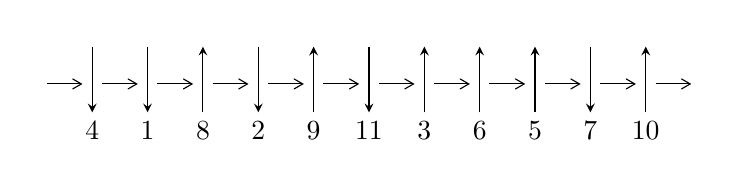
\begin{tikzpicture}[x=20pt, y=17pt]
	% nodes
	\node (C0) at (0, 0) {};
	\node (C1) at (1, 0) {};
	\node (C1U) at (1, +1) {};
	\node (C1D) at (1, -1) {4};

	\node (C2) at (2, 0) {};
	\node (C2U) at (2, +1) {};
	\node (C2D) at (2, -1) {1};

	\node (C3) at (3, 0) {};
	\node (C3U) at (3, +1) {};
	\node (C3D) at (3, -1) {8};

	\node (C4) at (4, 0) {};
	\node (C4U) at (4, +1) {};
	\node (C4D) at (4, -1) {2};

	\node (C5) at (5, 0) {};
	\node (C5U) at (5, +1) {};
	\node (C5D) at (5, -1) {9};

	\node (C6) at (6, 0) {};
	\node (C6U) at (6, +1) {};
	\node (C6D) at (6, -1) {11};

	\node (C7) at (7, 0) {};
	\node (C7U) at (7, +1) {};
	\node (C7D) at (7, -1) {3};

	\node (C8) at (8, 0) {};
	\node (C8U) at (8, +1) {};
	\node (C8D) at (8, -1) {6};

	\node (C9) at (9, 0) {};
	\node (C9U) at (9, +1) {};
	\node (C9D) at (9, -1) {5};

	\node (C10) at (10, 0) {};
	\node (C10U) at (10, +1) {};
	\node (C10D) at (10, -1) {7};

	\node (C11) at (11, 0) {};
	\node (C11U) at (11, +1) {};
	\node (C11D) at (11, -1) {10};
	\node (C12) at (12, 0) {};

	% arrows
	\draw[->,>={angle 60}]
	(C0) edge (C1) (C1) edge (C2) (C2) edge (C3) (C3) edge (C4) (C4) edge (C5) (C5) edge (C6) (C6) edge (C7) (C7) edge (C8) (C8) edge (C9) (C9) edge (C10) (C10) edge (C11) (C11) edge (C12) ;	\draw[->,>=stealth]
	(C1U) edge (C1D) (C2U) edge (C2D) (C3D) edge (C3U) (C4U) edge (C4D) (C5D) edge (C5U) (C6U) edge (C6D) (C7D) edge (C7U) (C8D) edge (C8U) (C9D) edge (C9U) (C10U) edge (C10D) (C11D) edge (C11U) ;
	\end{tikzpicture} \\
\hhline{~~} \\& 
\textbf{Solving Sequence} \\ \cline{2-2} 
 &
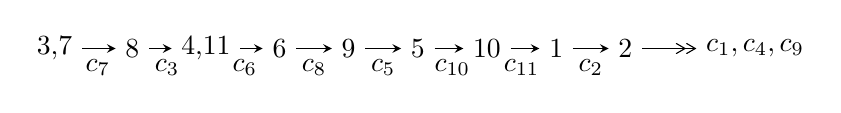
\begin{tikzpicture}[x=25pt, y=7pt]
	% node
	\node (A0) at (-1/8, 0) {3,7};
	\node (A1) at (1, 0) {8};
	\node (A2) at (33/16, 0) {4,11};
	\node (A3) at (25/8, 0) {6};
	\node (A4) at (33/8, 0) {9};
	\node (A5) at (41/8, 0) {5};
	\node (A6) at (49/8, 0) {10};
	\node (A7) at (57/8, 0) {1};
	\node (A8) at (65/8, 0) {2};
	\node (C1) at (1/2, -1) {$c_{7}$};
	\node (C2) at (3/2, -1) {$c_{3}$};
	\node (C3) at (21/8, -1) {$c_{6}$};
	\node (C4) at (29/8, -1) {$c_{8}$};
	\node (C5) at (37/8, -1) {$c_{5}$};
	\node (C6) at (45/8, -1) {$c_{10}$};
	\node (C7) at (53/8, -1) {$c_{11}$};
	\node (C8) at (61/8, -1) {$c_{2}$};
	\node (A9) at (10, 0) {$c_{1},c_{4},c_{9}$};

	% edge
	\draw[->,>=stealth]	
	(A0) edge (A1) (A1) edge (A2) (A2) edge (A3) (A3) edge (A4) (A4) edge (A5) (A5) edge (A6) (A6) edge (A7) (A7) edge (A8) ;
	\draw[->>,>={angle 60}]	
	(A8) edge (A9);
\end{tikzpicture} \\ 

\end{tabular} \\

\footnotetext{
The image of knot diagram is generated by the software ``\textbf{Draw programme}" developed by Andrew Bartholomew(\url{http://www.layer8.co.uk/maths/draw/index.htm\#Running-draw}), where we modified some parts for our purpose(\url{https://github.com/CATsTAILs/LinksPainter}).
}\phantom \\ \newline 
\centering \textbf{Ideals for irreducible components\footnotemark of $X_{\text{par}}$} 
 
\begin{align*}
I^u_{1}&=\langle 
1.39701\times10^{52} u^{49}-1.56890\times10^{52} u^{48}+\cdots+9.78680\times10^{53} b-2.06404\times10^{53},\\
\phantom{I^u_{1}}&\phantom{= \langle  }2.86648\times10^{52} u^{49}-4.68399\times10^{52} u^{48}+\cdots+9.78680\times10^{53} a-2.53995\times10^{54},\;u^{50}-2 u^{49}+\cdots-80 u+64\rangle \\
I^u_{2}&=\langle 
-36 u^5 a^2-80 u^4 a^2+64 u^3 a^2+36 u^5-7 a^2 u^2+80 u^4-40 a^2 u-64 u^3-22 a^2-276 u^2+283 b+40 u+22,\\
\phantom{I^u_{2}}&\phantom{= \langle  }2 u^5 a^2+u^5 a+\cdots- a-5,\;u^6+u^5- u^4-2 u^3+u+1\rangle \\
I^u_{3}&=\langle 
- u^5+2 u^3+b- u,\;u^4+2 u^3-3 u^2+a-3 u+2,\;u^6-3 u^4+2 u^2+1\rangle \\
\\
I^v_{1}&=\langle 
a,\;-2 v^3+3 v^2+4 b-8 v+3,\;2 v^4- v^3+5 v^2+v+1\rangle \\
\end{align*}
\raggedright * 4 irreducible components of $\dim_{\mathbb{C}}=0$, with total 78 representations.\\
\footnotetext{All coefficients of polynomials are rational numbers. But the coefficients are sometimes approximated in decimal forms when there is not enough margin.}
\newpage
\renewcommand{\arraystretch}{1}
\centering \section*{I. $I^u_{1}= \langle 1.40\times10^{52} u^{49}-1.57\times10^{52} u^{48}+\cdots+9.79\times10^{53} b-2.06\times10^{53},\;2.87\times10^{52} u^{49}-4.68\times10^{52} u^{48}+\cdots+9.79\times10^{53} a-2.54\times10^{54},\;u^{50}-2 u^{49}+\cdots-80 u+64 \rangle$}
\flushleft \textbf{(i) Arc colorings}\\
\begin{tabular}{m{7pt} m{180pt} m{7pt} m{180pt} }
\flushright $a_{3}=$&$\begin{pmatrix}0\\u\end{pmatrix}$ \\
\flushright $a_{7}=$&$\begin{pmatrix}1\\0\end{pmatrix}$ \\
\flushright $a_{8}=$&$\begin{pmatrix}1\\- u^2\end{pmatrix}$ \\
\flushright $a_{4}=$&$\begin{pmatrix}u\\- u^3+u\end{pmatrix}$ \\
\flushright $a_{11}=$&$\begin{pmatrix}-0.0292893 u^{49}+0.0478602 u^{48}+\cdots+0.349631 u+2.59529\\-0.0142744 u^{49}+0.0160307 u^{48}+\cdots-0.546290 u+0.210900\end{pmatrix}$ \\
\flushright $a_{6}=$&$\begin{pmatrix}0.0506276 u^{49}-0.0564076 u^{48}+\cdots+1.79590 u-3.09324\\-0.0101755 u^{49}+0.0132424 u^{48}+\cdots+0.365267 u+1.43307\end{pmatrix}$ \\
\flushright $a_{9}=$&$\begin{pmatrix}0.0251404 u^{49}-0.0341614 u^{48}+\cdots-0.178601 u-0.734921\\0.0178177 u^{49}-0.0204546 u^{48}+\cdots-0.655163 u+0.0702679\end{pmatrix}$ \\
\flushright $a_{5}=$&$\begin{pmatrix}0.0359682 u^{49}-0.0375079 u^{48}+\cdots+0.971454 u-2.70728\\-0.0171934 u^{49}+0.0404449 u^{48}+\cdots+1.08010 u+1.42517\end{pmatrix}$ \\
\flushright $a_{10}=$&$\begin{pmatrix}-0.0435637 u^{49}+0.0638909 u^{48}+\cdots-0.196658 u+2.80619\\-0.0142744 u^{49}+0.0160307 u^{48}+\cdots-0.546290 u+0.210900\end{pmatrix}$ \\
\flushright $a_{1}=$&$\begin{pmatrix}-0.0341694 u^{49}+0.0511276 u^{48}+\cdots+0.560955 u+1.92903\\0.00179875 u^{49}+0.0136197 u^{48}+\cdots+1.53241 u-0.778251\end{pmatrix}$ \\
\flushright $a_{2}=$&$\begin{pmatrix}-0.0608849 u^{49}+0.0808601 u^{48}+\cdots-0.638959 u+4.29539\\-0.0126196 u^{49}+0.0224728 u^{48}+\cdots+0.518576 u+0.0714096\end{pmatrix}$\\ \flushright $a_{2}=$&$\begin{pmatrix}-0.0608849 u^{49}+0.0808601 u^{48}+\cdots-0.638959 u+4.29539\\-0.0126196 u^{49}+0.0224728 u^{48}+\cdots+0.518576 u+0.0714096\end{pmatrix}$\\&\end{tabular}
\flushleft \textbf{(ii) Obstruction class $= -1$}\\~\\
\flushleft \textbf{(iii) Cusp Shapes $= -0.0626913 u^{49}+0.0376218 u^{48}+\cdots-2.19058 u+7.82840$}\\~\\
\newpage\renewcommand{\arraystretch}{1}
\flushleft \textbf{(iv) u-Polynomials at the component}\newline \\
\begin{tabular}{m{50pt}|m{274pt}}
Crossings & \hspace{64pt}u-Polynomials at each crossing \\
\hline $$\begin{aligned}c_{1},c_{4}\end{aligned}$$&$\begin{aligned}
&u^{50}-4 u^{49}+\cdots+3 u+4
\end{aligned}$\\
\hline $$\begin{aligned}c_{2}\end{aligned}$$&$\begin{aligned}
&u^{50}+24 u^{49}+\cdots-255 u+16
\end{aligned}$\\
\hline $$\begin{aligned}c_{3},c_{7}\end{aligned}$$&$\begin{aligned}
&u^{50}-2 u^{49}+\cdots-80 u+64
\end{aligned}$\\
\hline $$\begin{aligned}c_{5},c_{8},c_{9}\end{aligned}$$&$\begin{aligned}
&u^{50}+2 u^{49}+\cdots+76 u+17
\end{aligned}$\\
\hline $$\begin{aligned}c_{6},c_{10}\end{aligned}$$&$\begin{aligned}
&u^{50}+2 u^{49}+\cdots+72 u+17
\end{aligned}$\\
\hline $$\begin{aligned}c_{11}\end{aligned}$$&$\begin{aligned}
&u^{50}-20 u^{49}+\cdots-4370 u+289
\end{aligned}$\\
\hline
\end{tabular}\\~\\
\newpage\renewcommand{\arraystretch}{1}
\flushleft \textbf{(v) Riley Polynomials at the component}\newline \\
\begin{tabular}{m{50pt}|m{274pt}}
Crossings & \hspace{64pt}Riley Polynomials at each crossing \\
\hline $$\begin{aligned}c_{1},c_{4}\end{aligned}$$&$\begin{aligned}
&y^{50}-24 y^{49}+\cdots+255 y+16
\end{aligned}$\\
\hline $$\begin{aligned}c_{2}\end{aligned}$$&$\begin{aligned}
&y^{50}+8 y^{49}+\cdots+29791 y+256
\end{aligned}$\\
\hline $$\begin{aligned}c_{3},c_{7}\end{aligned}$$&$\begin{aligned}
&y^{50}-24 y^{49}+\cdots-19712 y+4096
\end{aligned}$\\
\hline $$\begin{aligned}c_{5},c_{8},c_{9}\end{aligned}$$&$\begin{aligned}
&y^{50}+52 y^{49}+\cdots-846 y+289
\end{aligned}$\\
\hline $$\begin{aligned}c_{6},c_{10}\end{aligned}$$&$\begin{aligned}
&y^{50}+20 y^{49}+\cdots+4370 y+289
\end{aligned}$\\
\hline $$\begin{aligned}c_{11}\end{aligned}$$&$\begin{aligned}
&y^{50}+28 y^{49}+\cdots-180694 y+83521
\end{aligned}$\\
\hline
\end{tabular}\\~\\
\newpage\flushleft \textbf{(vi) Complex Volumes and Cusp Shapes}
$$\begin{array}{c|c|c}  
\text{Solutions to }I^u_{1}& \I (\text{vol} + \sqrt{-1}CS) & \text{Cusp shape}\\
 \hline 
\begin{aligned}
u &= \phantom{-}0.907272 + 0.392918 I \\
a &= -0.420194 + 0.002697 I \\
b &= -0.699224 - 0.714437 I\end{aligned}
 & -0.744870 + 0.584560 I & \phantom{-}0.202019 - 0.958990 I \\ \hline\begin{aligned}
u &= \phantom{-}0.907272 - 0.392918 I \\
a &= -0.420194 - 0.002697 I \\
b &= -0.699224 + 0.714437 I\end{aligned}
 & -0.744870 - 0.584560 I & \phantom{-}0.202019 + 0.958990 I \\ \hline\begin{aligned}
u &= -0.936602 + 0.118293 I \\
a &= -0.318743 - 0.218959 I \\
b &= -0.620116 - 0.388367 I\end{aligned}
 & -0.08204 - 3.21276 I & \phantom{-}0.42949 + 6.66311 I \\ \hline\begin{aligned}
u &= -0.936602 - 0.118293 I \\
a &= -0.318743 + 0.218959 I \\
b &= -0.620116 + 0.388367 I\end{aligned}
 & -0.08204 + 3.21276 I & \phantom{-}0.42949 - 6.66311 I \\ \hline\begin{aligned}
u &= -0.473630 + 0.961275 I \\
a &= \phantom{-}0.323168 - 0.723326 I \\
b &= \phantom{-}0.711410 + 0.630048 I\end{aligned}
 & -5.28661 - 1.41187 I & -2.51524 + 3.36613 I \\ \hline\begin{aligned}
u &= -0.473630 - 0.961275 I \\
a &= \phantom{-}0.323168 + 0.723326 I \\
b &= \phantom{-}0.711410 - 0.630048 I\end{aligned}
 & -5.28661 + 1.41187 I & -2.51524 - 3.36613 I \\ \hline\begin{aligned}
u &= \phantom{-}0.449533 + 0.975399 I \\
a &= -0.509462 + 0.216523 I \\
b &= -0.517652 - 1.021650 I\end{aligned}
 & -0.28876 - 5.04770 I & \phantom{-}1.29595 + 6.45390 I \\ \hline\begin{aligned}
u &= \phantom{-}0.449533 - 0.975399 I \\
a &= -0.509462 - 0.216523 I \\
b &= -0.517652 + 1.021650 I\end{aligned}
 & -0.28876 + 5.04770 I & \phantom{-}1.29595 - 6.45390 I \\ \hline\begin{aligned}
u &= \phantom{-}0.815974 + 0.347535 I \\
a &= \phantom{-}1.49469 + 2.72833 I \\
b &= \phantom{-}0.468151 - 0.953658 I\end{aligned}
 & -1.11120 + 2.63706 I & \phantom{-}2.56560 - 6.52941 I \\ \hline\begin{aligned}
u &= \phantom{-}0.815974 - 0.347535 I \\
a &= \phantom{-}1.49469 - 2.72833 I \\
b &= \phantom{-}0.468151 + 0.953658 I\end{aligned}
 & -1.11120 - 2.63706 I & \phantom{-}2.56560 + 6.52941 I\\
 \hline 
 \end{array}$$\newpage$$\begin{array}{c|c|c}  
\text{Solutions to }I^u_{1}& \I (\text{vol} + \sqrt{-1}CS) & \text{Cusp shape}\\
 \hline 
\begin{aligned}
u &= \phantom{-}0.697235 + 0.535365 I \\
a &= \phantom{-}0.315606 + 0.602693 I \\
b &= \phantom{-}0.954432 - 0.777792 I\end{aligned}
 & -9.12170 + 4.13349 I & -4.37982 - 7.84583 I \\ \hline\begin{aligned}
u &= \phantom{-}0.697235 - 0.535365 I \\
a &= \phantom{-}0.315606 - 0.602693 I \\
b &= \phantom{-}0.954432 + 0.777792 I\end{aligned}
 & -9.12170 - 4.13349 I & -4.37982 + 7.84583 I \\ \hline\begin{aligned}
u &= \phantom{-}0.953458 + 0.598229 I \\
a &= \phantom{-}0.949740 - 0.081078 I \\
b &= -0.813160 - 0.543764 I\end{aligned}
 & -8.29977 + 0.42603 I & -4.99238 - 0.29759 I \\ \hline\begin{aligned}
u &= \phantom{-}0.953458 - 0.598229 I \\
a &= \phantom{-}0.949740 + 0.081078 I \\
b &= -0.813160 + 0.543764 I\end{aligned}
 & -8.29977 - 0.42603 I & -4.99238 + 0.29759 I \\ \hline\begin{aligned}
u &= -0.024298 + 0.854586 I \\
a &= -0.679350 - 0.293209 I \\
b &= -0.329331 + 0.976215 I\end{aligned}
 & \phantom{-}0.969303 + 1.022450 I & \phantom{-}4.86262 - 1.22345 I \\ \hline\begin{aligned}
u &= -0.024298 - 0.854586 I \\
a &= -0.679350 + 0.293209 I \\
b &= -0.329331 - 0.976215 I\end{aligned}
 & \phantom{-}0.969303 - 1.022450 I & \phantom{-}4.86262 + 1.22345 I \\ \hline\begin{aligned}
u &= \phantom{-}0.232434 + 1.128490 I \\
a &= \phantom{-}0.171601 - 0.671528 I \\
b &= \phantom{-}0.613539 + 0.992173 I\end{aligned}
 & -4.19193 - 3.67253 I & -1.22751 + 2.31471 I \\ \hline\begin{aligned}
u &= \phantom{-}0.232434 - 1.128490 I \\
a &= \phantom{-}0.171601 + 0.671528 I \\
b &= \phantom{-}0.613539 - 0.992173 I\end{aligned}
 & -4.19193 + 3.67253 I & -1.22751 - 2.31471 I \\ \hline\begin{aligned}
u &= -1.083130 + 0.424102 I \\
a &= -0.51370 + 2.44482 I \\
b &= -0.653200 - 1.057010 I\end{aligned}
 & -6.75514 - 5.91277 I & -2.21392 + 5.18403 I \\ \hline\begin{aligned}
u &= -1.083130 - 0.424102 I \\
a &= -0.51370 - 2.44482 I \\
b &= -0.653200 + 1.057010 I\end{aligned}
 & -6.75514 + 5.91277 I & -2.21392 - 5.18403 I\\
 \hline 
 \end{array}$$\newpage$$\begin{array}{c|c|c}  
\text{Solutions to }I^u_{1}& \I (\text{vol} + \sqrt{-1}CS) & \text{Cusp shape}\\
 \hline 
\begin{aligned}
u &= \phantom{-}0.643203 + 1.007070 I \\
a &= \phantom{-}0.426141 + 0.701622 I \\
b &= \phantom{-}0.850297 - 0.462719 I\end{aligned}
 & -7.77183 - 3.25304 I & -5.27621 + 1.64998 I \\ \hline\begin{aligned}
u &= \phantom{-}0.643203 - 1.007070 I \\
a &= \phantom{-}0.426141 - 0.701622 I \\
b &= \phantom{-}0.850297 + 0.462719 I\end{aligned}
 & -7.77183 + 3.25304 I & -5.27621 - 1.64998 I \\ \hline\begin{aligned}
u &= -1.089060 + 0.646090 I \\
a &= \phantom{-}0.400714 + 0.040363 I \\
b &= -0.874960 + 0.339779 I\end{aligned}
 & -3.37785 - 4.34752 I & -0.97473 + 2.40737 I \\ \hline\begin{aligned}
u &= -1.089060 - 0.646090 I \\
a &= \phantom{-}0.400714 - 0.040363 I \\
b &= -0.874960 - 0.339779 I\end{aligned}
 & -3.37785 + 4.34752 I & -0.97473 - 2.40737 I \\ \hline\begin{aligned}
u &= -0.538092 + 1.149580 I \\
a &= \phantom{-}0.144817 + 0.630742 I \\
b &= \phantom{-}0.646329 - 1.107890 I\end{aligned}
 & -5.83333 + 8.80963 I & -2.37769 - 6.43347 I \\ \hline\begin{aligned}
u &= -0.538092 - 1.149580 I \\
a &= \phantom{-}0.144817 - 0.630742 I \\
b &= \phantom{-}0.646329 + 1.107890 I\end{aligned}
 & -5.83333 - 8.80963 I & -2.37769 + 6.43347 I \\ \hline\begin{aligned}
u &= -1.174390 + 0.484424 I \\
a &= \phantom{-}0.96122 - 1.70050 I \\
b &= \phantom{-}0.536868 + 1.111540 I\end{aligned}
 & \phantom{-}4.31618 - 5.59634 I & \phantom{-}6.06047 + 4.87396 I \\ \hline\begin{aligned}
u &= -1.174390 - 0.484424 I \\
a &= \phantom{-}0.96122 + 1.70050 I \\
b &= \phantom{-}0.536868 - 1.111540 I\end{aligned}
 & \phantom{-}4.31618 + 5.59634 I & \phantom{-}6.06047 - 4.87396 I \\ \hline\begin{aligned}
u &= -1.266720 + 0.096929 I \\
a &= -0.02752 + 1.80946 I \\
b &= \phantom{-}0.280639 - 1.152600 I\end{aligned}
 & \phantom{-}6.04456 + 2.16278 I & \phantom{-}8.79757 - 2.89733 I \\ \hline\begin{aligned}
u &= -1.266720 - 0.096929 I \\
a &= -0.02752 - 1.80946 I \\
b &= \phantom{-}0.280639 + 1.152600 I\end{aligned}
 & \phantom{-}6.04456 - 2.16278 I & \phantom{-}8.79757 + 2.89733 I\\
 \hline 
 \end{array}$$\newpage$$\begin{array}{c|c|c}  
\text{Solutions to }I^u_{1}& \I (\text{vol} + \sqrt{-1}CS) & \text{Cusp shape}\\
 \hline 
\begin{aligned}
u &= -0.595443 + 0.355867 I \\
a &= \phantom{-}0.228768 + 0.590040 I \\
b &= \phantom{-}0.871755 - 0.998829 I\end{aligned}
 & -8.47083 + 2.48602 I & -1.45090 + 5.51453 I \\ \hline\begin{aligned}
u &= -0.595443 - 0.355867 I \\
a &= \phantom{-}0.228768 - 0.590040 I \\
b &= \phantom{-}0.871755 + 0.998829 I\end{aligned}
 & -8.47083 - 2.48602 I & -1.45090 - 5.51453 I \\ \hline\begin{aligned}
u &= \phantom{-}1.264420 + 0.377230 I \\
a &= -0.33373 - 1.58630 I \\
b &= \phantom{-}0.170537 + 1.148410 I\end{aligned}
 & \phantom{-}5.10728 + 3.38490 I & \phantom{-}7.93360 - 3.33034 I \\ \hline\begin{aligned}
u &= \phantom{-}1.264420 - 0.377230 I \\
a &= -0.33373 + 1.58630 I \\
b &= \phantom{-}0.170537 - 1.148410 I\end{aligned}
 & \phantom{-}5.10728 - 3.38490 I & \phantom{-}7.93360 + 3.33034 I \\ \hline\begin{aligned}
u &= \phantom{-}1.117610 + 0.748018 I \\
a &= \phantom{-}0.293611 - 0.238740 I \\
b &= -1.007530 - 0.362892 I\end{aligned}
 & -6.21564 + 9.65095 I & \phantom{-0.000000 } 0. - 5.84415 I \\ \hline\begin{aligned}
u &= \phantom{-}1.117610 - 0.748018 I \\
a &= \phantom{-}0.293611 + 0.238740 I \\
b &= -1.007530 + 0.362892 I\end{aligned}
 & -6.21564 - 9.65095 I & \phantom{-0.000000 -}0. + 5.84415 I \\ \hline\begin{aligned}
u &= \phantom{-}1.175850 + 0.667191 I \\
a &= \phantom{-}1.12100 + 1.42946 I \\
b &= \phantom{-}0.621576 - 1.109980 I\end{aligned}
 & \phantom{-}1.99477 + 11.04250 I & \phantom{-0.000000 } 0. - 8.76647 I \\ \hline\begin{aligned}
u &= \phantom{-}1.175850 - 0.667191 I \\
a &= \phantom{-}1.12100 - 1.42946 I \\
b &= \phantom{-}0.621576 + 1.109980 I\end{aligned}
 & \phantom{-}1.99477 - 11.04250 I & \phantom{-0.000000 -}0. + 8.76647 I \\ \hline\begin{aligned}
u &= -0.399787 + 0.467256 I \\
a &= -1.67834 - 1.67643 I \\
b &= \phantom{-}0.114999 - 0.542444 I\end{aligned}
 & -1.97039 + 0.78230 I & -5.45253 + 2.09256 I \\ \hline\begin{aligned}
u &= -0.399787 - 0.467256 I \\
a &= -1.67834 + 1.67643 I \\
b &= \phantom{-}0.114999 + 0.542444 I\end{aligned}
 & -1.97039 - 0.78230 I & -5.45253 - 2.09256 I\\
 \hline 
 \end{array}$$\newpage$$\begin{array}{c|c|c}  
\text{Solutions to }I^u_{1}& \I (\text{vol} + \sqrt{-1}CS) & \text{Cusp shape}\\
 \hline 
\begin{aligned}
u &= \phantom{-}1.27251 + 0.63129 I \\
a &= -0.67000 - 1.80811 I \\
b &= -0.616422 + 1.164310 I\end{aligned}
 & -0.91239 + 9.84583 I & \phantom{-0.000000 } 0 \\ \hline\begin{aligned}
u &= \phantom{-}1.27251 - 0.63129 I \\
a &= -0.67000 + 1.80811 I \\
b &= -0.616422 - 1.164310 I\end{aligned}
 & -0.91239 - 9.84583 I & \phantom{-0.000000 } 0 \\ \hline\begin{aligned}
u &= -1.22350 + 0.76980 I \\
a &= -0.88939 + 1.67143 I \\
b &= -0.662987 - 1.206930 I\end{aligned}
 & -3.6196 - 15.6826 I & \phantom{-0.000000 } 0 \\ \hline\begin{aligned}
u &= -1.22350 - 0.76980 I \\
a &= -0.88939 - 1.67143 I \\
b &= -0.662987 + 1.206930 I\end{aligned}
 & -3.6196 + 15.6826 I & \phantom{-0.000000 } 0 \\ \hline\begin{aligned}
u &= \phantom{-}0.257076 + 0.420882 I \\
a &= -0.990050 - 0.003127 I \\
b &= -0.223361 + 0.753004 I\end{aligned}
 & \phantom{-}0.426067 + 1.178950 I & \phantom{-}4.63590 - 6.06198 I \\ \hline\begin{aligned}
u &= \phantom{-}0.257076 - 0.420882 I \\
a &= -0.990050 + 0.003127 I \\
b &= -0.223361 - 0.753004 I\end{aligned}
 & \phantom{-}0.426067 - 1.178950 I & \phantom{-}4.63590 + 6.06198 I \\ \hline\begin{aligned}
u &= \phantom{-}1.51280 + 0.01490 I \\
a &= \phantom{-}0.22721 - 1.58372 I \\
b &= -0.435520 + 0.951672 I\end{aligned}
 & \phantom{-}2.35249 + 4.91231 I & \phantom{-0.000000 } 0 \\ \hline\begin{aligned}
u &= \phantom{-}1.51280 - 0.01490 I \\
a &= \phantom{-}0.22721 + 1.58372 I \\
b &= -0.435520 - 0.951672 I\end{aligned}
 & \phantom{-}2.35249 - 4.91231 I & \phantom{-0.000000 } 0 \\ \hline\begin{aligned}
u &= -1.49474 + 0.29701 I \\
a &= \phantom{-}0.409690 - 1.327970 I \\
b &= -0.387075 + 0.830148 I\end{aligned}
 & \phantom{-}1.85024 - 1.51739 I & \phantom{-0.000000 } 0 \\ \hline\begin{aligned}
u &= -1.49474 - 0.29701 I \\
a &= \phantom{-}0.409690 + 1.327970 I \\
b &= -0.387075 - 0.830148 I\end{aligned}
 & \phantom{-}1.85024 + 1.51739 I & \phantom{-0.000000 } 0\\
 \hline 
 \end{array}$$\newpage\newpage\renewcommand{\arraystretch}{1}
\centering \section*{II. $I^u_{2}= \langle -36 u^5 a^2+36 u^5+\cdots-22 a^2+22,\;2 u^5 a^2+u^5 a+\cdots- a-5,\;u^6+u^5- u^4-2 u^3+u+1 \rangle$}
\flushleft \textbf{(i) Arc colorings}\\
\begin{tabular}{m{7pt} m{180pt} m{7pt} m{180pt} }
\flushright $a_{3}=$&$\begin{pmatrix}0\\u\end{pmatrix}$ \\
\flushright $a_{7}=$&$\begin{pmatrix}1\\0\end{pmatrix}$ \\
\flushright $a_{8}=$&$\begin{pmatrix}1\\- u^2\end{pmatrix}$ \\
\flushright $a_{4}=$&$\begin{pmatrix}u\\- u^3+u\end{pmatrix}$ \\
\flushright $a_{11}=$&$\begin{pmatrix}a\\0.127208 a^{2} u^{5}-0.127208 u^{5}+\cdots+0.0777385 a^{2}-0.0777385\end{pmatrix}$ \\
\flushright $a_{6}=$&$\begin{pmatrix}-0.127208 a^{2} u^{5}+0.127208 u^{5}+\cdots+a+2.07774\\-0.127208 a^{2} u^{5}+0.127208 u^{5}+\cdots-0.0777385 a^{2}+0.0777385\end{pmatrix}$ \\
\flushright $a_{9}=$&$\begin{pmatrix}- a\\-0.127208 a^{2} u^{5}+0.127208 u^{5}+\cdots-0.0777385 a^{2}+0.0777385\end{pmatrix}$ \\
\flushright $a_{5}=$&$\begin{pmatrix}1\\0\end{pmatrix}$ \\
\flushright $a_{10}=$&$\begin{pmatrix}0.127208 a^{2} u^{5}-0.127208 u^{5}+\cdots+a-0.0777385\\0.127208 a^{2} u^{5}-0.127208 u^{5}+\cdots+0.0777385 a^{2}-0.0777385\end{pmatrix}$ \\
\flushright $a_{1}=$&$\begin{pmatrix}u^2-1\\u^2\end{pmatrix}$ \\
\flushright $a_{2}=$&$\begin{pmatrix}u^5-2 u^3+u\\u^5- u^3+u\end{pmatrix}$\\ \flushright $a_{2}=$&$\begin{pmatrix}u^5-2 u^3+u\\u^5- u^3+u\end{pmatrix}$\\&\end{tabular}
\flushleft \textbf{(ii) Obstruction class $= -1$}\\~\\
\flushleft \textbf{(iii) Cusp Shapes $= -4 u^4+4 u^2+4 u-2$}\\~\\
\newpage\renewcommand{\arraystretch}{1}
\flushleft \textbf{(iv) u-Polynomials at the component}\newline \\
\begin{tabular}{m{50pt}|m{274pt}}
Crossings & \hspace{64pt}u-Polynomials at each crossing \\
\hline $$\begin{aligned}c_{1},c_{4}\end{aligned}$$&$\begin{aligned}
&(u^6- u^5- u^4+2 u^3- u+1)^3
\end{aligned}$\\
\hline $$\begin{aligned}c_{2}\end{aligned}$$&$\begin{aligned}
&(u^6+3 u^5+5 u^4+4 u^3+2 u^2+u+1)^3
\end{aligned}$\\
\hline $$\begin{aligned}c_{3},c_{7}\end{aligned}$$&$\begin{aligned}
&(u^6+u^5- u^4-2 u^3+u+1)^3
\end{aligned}$\\
\hline $$\begin{aligned}c_{5},c_{6},c_{8}\\c_{9},c_{10}\end{aligned}$$&$\begin{aligned}
&u^{18}+6 u^{16}+\cdots- u+1
\end{aligned}$\\
\hline $$\begin{aligned}c_{11}\end{aligned}$$&$\begin{aligned}
&u^{18}-12 u^{17}+\cdots-3 u+1
\end{aligned}$\\
\hline
\end{tabular}\\~\\
\newpage\renewcommand{\arraystretch}{1}
\flushleft \textbf{(v) Riley Polynomials at the component}\newline \\
\begin{tabular}{m{50pt}|m{274pt}}
Crossings & \hspace{64pt}Riley Polynomials at each crossing \\
\hline $$\begin{aligned}c_{1},c_{3},c_{4}\\c_{7}\end{aligned}$$&$\begin{aligned}
&(y^6-3 y^5+5 y^4-4 y^3+2 y^2- y+1)^3
\end{aligned}$\\
\hline $$\begin{aligned}c_{2}\end{aligned}$$&$\begin{aligned}
&(y^6+y^5+5 y^4+6 y^2+3 y+1)^3
\end{aligned}$\\
\hline $$\begin{aligned}c_{5},c_{6},c_{8}\\c_{9},c_{10}\end{aligned}$$&$\begin{aligned}
&y^{18}+12 y^{17}+\cdots+3 y+1
\end{aligned}$\\
\hline $$\begin{aligned}c_{11}\end{aligned}$$&$\begin{aligned}
&y^{18}-12 y^{17}+\cdots+15 y+1
\end{aligned}$\\
\hline
\end{tabular}\\~\\
\newpage\flushleft \textbf{(vi) Complex Volumes and Cusp Shapes}
$$\begin{array}{c|c|c}  
\text{Solutions to }I^u_{2}& \I (\text{vol} + \sqrt{-1}CS) & \text{Cusp shape}\\
 \hline 
\begin{aligned}
u &= \phantom{-}1.002190 + 0.295542 I \\
a &= -0.158981 + 0.210049 I \\
b &= \phantom{-}0.700352 + 0.245687 I\end{aligned}
 & \phantom{-}1.89061 + 0.92430 I & \phantom{-}3.71672 - 0.79423 I \\ \hline\begin{aligned}
u &= \phantom{-}1.002190 + 0.295542 I \\
a &= -1.28821 - 1.33402 I \\
b &= -0.461864 + 1.032610 I\end{aligned}
 & \phantom{-}1.89061 + 0.92430 I & \phantom{-}3.71672 - 0.79423 I \\ \hline\begin{aligned}
u &= \phantom{-}1.002190 + 0.295542 I \\
a &= -0.09163 + 2.11799 I \\
b &= -0.238488 - 1.278300 I\end{aligned}
 & \phantom{-}1.89061 + 0.92430 I & \phantom{-}3.71672 - 0.79423 I \\ \hline\begin{aligned}
u &= \phantom{-}1.002190 - 0.295542 I \\
a &= -0.158981 - 0.210049 I \\
b &= \phantom{-}0.700352 - 0.245687 I\end{aligned}
 & \phantom{-}1.89061 - 0.92430 I & \phantom{-}3.71672 + 0.79423 I \\ \hline\begin{aligned}
u &= \phantom{-}1.002190 - 0.295542 I \\
a &= -1.28821 + 1.33402 I \\
b &= -0.461864 - 1.032610 I\end{aligned}
 & \phantom{-}1.89061 - 0.92430 I & \phantom{-}3.71672 + 0.79423 I \\ \hline\begin{aligned}
u &= \phantom{-}1.002190 - 0.295542 I \\
a &= -0.09163 - 2.11799 I \\
b &= -0.238488 + 1.278300 I\end{aligned}
 & \phantom{-}1.89061 - 0.92430 I & \phantom{-}3.71672 + 0.79423 I \\ \hline\begin{aligned}
u &= -0.428243 + 0.664531 I \\
a &= -1.404780 + 0.070635 I \\
b &= -0.414097 - 0.427367 I\end{aligned}
 & -1.89061 + 0.92430 I & -3.71672 - 0.79423 I \\ \hline\begin{aligned}
u &= -0.428243 + 0.664531 I \\
a &= \phantom{-}0.19096 - 1.40605 I \\
b &= \phantom{-}0.339178 - 0.790848 I\end{aligned}
 & -1.89061 + 0.92430 I & -3.71672 - 0.79423 I \\ \hline\begin{aligned}
u &= -0.428243 + 0.664531 I \\
a &= \phantom{-}2.53589 - 1.57875 I \\
b &= \phantom{-}0.074919 + 1.218220 I\end{aligned}
 & -1.89061 + 0.92430 I & -3.71672 - 0.79423 I \\ \hline\begin{aligned}
u &= -0.428243 - 0.664531 I \\
a &= -1.404780 - 0.070635 I \\
b &= -0.414097 + 0.427367 I\end{aligned}
 & -1.89061 - 0.92430 I & -3.71672 + 0.79423 I\\
 \hline 
 \end{array}$$\newpage$$\begin{array}{c|c|c}  
\text{Solutions to }I^u_{2}& \I (\text{vol} + \sqrt{-1}CS) & \text{Cusp shape}\\
 \hline 
\begin{aligned}
u &= -0.428243 - 0.664531 I \\
a &= \phantom{-}0.19096 + 1.40605 I \\
b &= \phantom{-}0.339178 + 0.790848 I\end{aligned}
 & -1.89061 - 0.92430 I & -3.71672 + 0.79423 I \\ \hline\begin{aligned}
u &= -0.428243 - 0.664531 I \\
a &= \phantom{-}2.53589 + 1.57875 I \\
b &= \phantom{-}0.074919 - 1.218220 I\end{aligned}
 & -1.89061 - 0.92430 I & -3.71672 + 0.79423 I \\ \hline\begin{aligned}
u &= -1.073950 + 0.558752 I \\
a &= -1.16030 + 0.89772 I \\
b &= -0.624190 - 0.955200 I\end{aligned}
 & \phantom{-0.000000 } -5.69302 I & \phantom{-0.000000 -}0. + 5.51057 I \\ \hline\begin{aligned}
u &= -1.073950 + 0.558752 I \\
a &= \phantom{-}0.008039 - 0.301999 I \\
b &= \phantom{-}0.798654 - 0.441445 I\end{aligned}
 & \phantom{-0.000000 } -5.69302 I & \phantom{-0.000000 -}0. + 5.51057 I \\ \hline\begin{aligned}
u &= -1.073950 + 0.558752 I \\
a &= \phantom{-}0.36901 - 1.71323 I \\
b &= -0.174464 + 1.396650 I\end{aligned}
 & \phantom{-0.000000 } -5.69302 I & \phantom{-0.000000 -}0. + 5.51057 I \\ \hline\begin{aligned}
u &= -1.073950 - 0.558752 I \\
a &= -1.16030 - 0.89772 I \\
b &= -0.624190 + 0.955200 I\end{aligned}
 & \phantom{-0.000000 -}5.69302 I & \phantom{-0.000000 } 0. - 5.51057 I \\ \hline\begin{aligned}
u &= -1.073950 - 0.558752 I \\
a &= \phantom{-}0.008039 + 0.301999 I \\
b &= \phantom{-}0.798654 + 0.441445 I\end{aligned}
 & \phantom{-0.000000 -}5.69302 I & \phantom{-0.000000 } 0. - 5.51057 I \\ \hline\begin{aligned}
u &= -1.073950 - 0.558752 I \\
a &= \phantom{-}0.36901 + 1.71323 I \\
b &= -0.174464 - 1.396650 I\end{aligned}
 & \phantom{-0.000000 -}5.69302 I & \phantom{-0.000000 } 0. - 5.51057 I\\
 \hline 
 \end{array}$$\newpage\newpage\renewcommand{\arraystretch}{1}
\centering \section*{III. $I^u_{3}= \langle - u^5+2 u^3+b- u,\;u^4+2 u^3-3 u^2+a-3 u+2,\;u^6-3 u^4+2 u^2+1 \rangle$}
\flushleft \textbf{(i) Arc colorings}\\
\begin{tabular}{m{7pt} m{180pt} m{7pt} m{180pt} }
\flushright $a_{3}=$&$\begin{pmatrix}0\\u\end{pmatrix}$ \\
\flushright $a_{7}=$&$\begin{pmatrix}1\\0\end{pmatrix}$ \\
\flushright $a_{8}=$&$\begin{pmatrix}1\\- u^2\end{pmatrix}$ \\
\flushright $a_{4}=$&$\begin{pmatrix}u\\- u^3+u\end{pmatrix}$ \\
\flushright $a_{11}=$&$\begin{pmatrix}- u^4-2 u^3+3 u^2+3 u-2\\u^5-2 u^3+u\end{pmatrix}$ \\
\flushright $a_{6}=$&$\begin{pmatrix}u^5+u^4-4 u^3-3 u^2+4 u+2\\1\end{pmatrix}$ \\
\flushright $a_{9}=$&$\begin{pmatrix}u^5- u^4-4 u^3+3 u^2+4 u-1\\u^5-2 u^3- u^2+u\end{pmatrix}$ \\
\flushright $a_{5}=$&$\begin{pmatrix}u^5-2 u^3+u\\- u^5+u^3+u\end{pmatrix}$ \\
\flushright $a_{10}=$&$\begin{pmatrix}u^5- u^4-4 u^3+3 u^2+4 u-2\\u^5-2 u^3+u\end{pmatrix}$ \\
\flushright $a_{1}=$&$\begin{pmatrix}- u^5+2 u^3- u\\0\end{pmatrix}$ \\
\flushright $a_{2}=$&$\begin{pmatrix}- u\\u\end{pmatrix}$\\ \flushright $a_{2}=$&$\begin{pmatrix}- u\\u\end{pmatrix}$\\&\end{tabular}
\flushleft \textbf{(ii) Obstruction class $= 1$}\\~\\
\flushleft \textbf{(iii) Cusp Shapes $= -4 u^4+8 u^2$}\\~\\
\newpage\renewcommand{\arraystretch}{1}
\flushleft \textbf{(iv) u-Polynomials at the component}\newline \\
\begin{tabular}{m{50pt}|m{274pt}}
Crossings & \hspace{64pt}u-Polynomials at each crossing \\
\hline $$\begin{aligned}c_{1}\end{aligned}$$&$\begin{aligned}
&(u^3+u^2-1)^2
\end{aligned}$\\
\hline $$\begin{aligned}c_{2}\end{aligned}$$&$\begin{aligned}
&(u^3+u^2+2 u+1)^2
\end{aligned}$\\
\hline $$\begin{aligned}c_{3},c_{7}\end{aligned}$$&$\begin{aligned}
&u^6-3 u^4+2 u^2+1
\end{aligned}$\\
\hline $$\begin{aligned}c_{4}\end{aligned}$$&$\begin{aligned}
&(u^3- u^2+1)^2
\end{aligned}$\\
\hline $$\begin{aligned}c_{5},c_{6},c_{8}\\c_{9},c_{10}\end{aligned}$$&$\begin{aligned}
&(u^2+1)^3
\end{aligned}$\\
\hline $$\begin{aligned}c_{11}\end{aligned}$$&$\begin{aligned}
&(u-1)^6
\end{aligned}$\\
\hline
\end{tabular}\\~\\
\newpage\renewcommand{\arraystretch}{1}
\flushleft \textbf{(v) Riley Polynomials at the component}\newline \\
\begin{tabular}{m{50pt}|m{274pt}}
Crossings & \hspace{64pt}Riley Polynomials at each crossing \\
\hline $$\begin{aligned}c_{1},c_{4}\end{aligned}$$&$\begin{aligned}
&(y^3- y^2+2 y-1)^2
\end{aligned}$\\
\hline $$\begin{aligned}c_{2}\end{aligned}$$&$\begin{aligned}
&(y^3+3 y^2+2 y-1)^2
\end{aligned}$\\
\hline $$\begin{aligned}c_{3},c_{7}\end{aligned}$$&$\begin{aligned}
&(y^3-3 y^2+2 y+1)^2
\end{aligned}$\\
\hline $$\begin{aligned}c_{5},c_{6},c_{8}\\c_{9},c_{10}\end{aligned}$$&$\begin{aligned}
&(y+1)^6
\end{aligned}$\\
\hline $$\begin{aligned}c_{11}\end{aligned}$$&$\begin{aligned}
&(y-1)^6
\end{aligned}$\\
\hline
\end{tabular}\\~\\
\newpage\flushleft \textbf{(vi) Complex Volumes and Cusp Shapes}
$$\begin{array}{c|c|c}  
\text{Solutions to }I^u_{3}& \I (\text{vol} + \sqrt{-1}CS) & \text{Cusp shape}\\
 \hline 
\begin{aligned}
u &= \phantom{-}1.307140 + 0.215080 I \\
a &= \phantom{-}0.35722 - 1.72238 I \\
b &= \phantom{-0.000000 -}1.000000 I\end{aligned}
 & \phantom{-}3.02413 + 2.82812 I & \phantom{-}3.50976 - 2.97945 I \\ \hline\begin{aligned}
u &= \phantom{-}1.307140 - 0.215080 I \\
a &= \phantom{-}0.35722 + 1.72238 I \\
b &= \phantom{-0.000000 } -1.000000 I\end{aligned}
 & \phantom{-}3.02413 - 2.82812 I & \phantom{-}3.50976 + 2.97945 I \\ \hline\begin{aligned}
u &= -1.307140 + 0.215080 I \\
a &= \phantom{-}0.72238 - 1.35722 I \\
b &= \phantom{-0.000000 -}1.000000 I\end{aligned}
 & \phantom{-}3.02413 - 2.82812 I & \phantom{-}3.50976 + 2.97945 I \\ \hline\begin{aligned}
u &= -1.307140 - 0.215080 I \\
a &= \phantom{-}0.72238 + 1.35722 I \\
b &= \phantom{-0.000000 } -1.000000 I\end{aligned}
 & \phantom{-}3.02413 + 2.82812 I & \phantom{-}3.50976 - 2.97945 I \\ \hline\begin{aligned}
u &= \phantom{-0.000000 -}0.569840 I \\
a &= -3.07960 + 2.07960 I \\
b &= \phantom{-0.000000 -}1.000000 I\end{aligned}
 & -1.11345\phantom{ +0.000000I} & -3.01950\phantom{ +0.000000I} \\ \hline\begin{aligned}
u &= \phantom{-0.000000 } -0.569840 I \\
a &= -3.07960 - 2.07960 I \\
b &= \phantom{-0.000000 } -1.000000 I\end{aligned}
 & -1.11345\phantom{ +0.000000I} & -3.01950\phantom{ +0.000000I}\\
 \hline 
 \end{array}$$\newpage\newpage\renewcommand{\arraystretch}{1}
\centering \section*{IV. $I^v_{1}= \langle a,\;-2 v^3+3 v^2+4 b-8 v+3,\;2 v^4- v^3+5 v^2+v+1 \rangle$}
\flushleft \textbf{(i) Arc colorings}\\
\begin{tabular}{m{7pt} m{180pt} m{7pt} m{180pt} }
\flushright $a_{3}=$&$\begin{pmatrix}v\\0\end{pmatrix}$ \\
\flushright $a_{7}=$&$\begin{pmatrix}1\\0\end{pmatrix}$ \\
\flushright $a_{8}=$&$\begin{pmatrix}1\\0\end{pmatrix}$ \\
\flushright $a_{4}=$&$\begin{pmatrix}v\\0\end{pmatrix}$ \\
\flushright $a_{11}=$&$\begin{pmatrix}0\\\frac{1}{2} v^3-\frac{3}{4} v^2+2 v-\frac{3}{4}\end{pmatrix}$ \\
\flushright $a_{6}=$&$\begin{pmatrix}1\\\frac{3}{2} v^3-\frac{5}{4} v^2+\frac{7}{2} v+\frac{1}{4}\end{pmatrix}$ \\
\flushright $a_{9}=$&$\begin{pmatrix}-\frac{3}{2} v^3+\frac{5}{4} v^2-\frac{7}{2} v+\frac{3}{4}\\v^2-\frac{1}{2} v+\frac{5}{2}\end{pmatrix}$ \\
\flushright $a_{5}=$&$\begin{pmatrix}-\frac{3}{2} v^3+\frac{1}{4} v^2-3 v-\frac{7}{4}\\-2 v^3+v^2-5 v-1\end{pmatrix}$ \\
\flushright $a_{10}=$&$\begin{pmatrix}\frac{1}{2} v^3-\frac{3}{4} v^2+2 v-\frac{3}{4}\\\frac{1}{2} v^3-\frac{3}{4} v^2+2 v-\frac{3}{4}\end{pmatrix}$ \\
\flushright $a_{1}=$&$\begin{pmatrix}\frac{3}{2} v^3-\frac{1}{4} v^2+3 v+\frac{7}{4}\\2 v^3- v^2+5 v+1\end{pmatrix}$ \\
\flushright $a_{2}=$&$\begin{pmatrix}\frac{3}{2} v^3-\frac{1}{4} v^2+4 v+\frac{7}{4}\\2 v^3- v^2+5 v+1\end{pmatrix}$\\ \flushright $a_{2}=$&$\begin{pmatrix}\frac{3}{2} v^3-\frac{1}{4} v^2+4 v+\frac{7}{4}\\2 v^3- v^2+5 v+1\end{pmatrix}$\\&\end{tabular}
\flushleft \textbf{(ii) Obstruction class $= 1$}\\~\\
\flushleft \textbf{(iii) Cusp Shapes $= -6 v^3+4 v^2-12 v-2$}\\~\\
\newpage\renewcommand{\arraystretch}{1}
\flushleft \textbf{(iv) u-Polynomials at the component}\newline \\
\begin{tabular}{m{50pt}|m{274pt}}
Crossings & \hspace{64pt}u-Polynomials at each crossing \\
\hline $$\begin{aligned}c_{1}\end{aligned}$$&$\begin{aligned}
&(u-1)^4
\end{aligned}$\\
\hline $$\begin{aligned}c_{2},c_{4}\end{aligned}$$&$\begin{aligned}
&(u+1)^4
\end{aligned}$\\
\hline $$\begin{aligned}c_{3},c_{7}\end{aligned}$$&$\begin{aligned}
&u^4
\end{aligned}$\\
\hline $$\begin{aligned}c_{5}\end{aligned}$$&$\begin{aligned}
&u^4+u^3+3 u^2+2 u+1
\end{aligned}$\\
\hline $$\begin{aligned}c_{6}\end{aligned}$$&$\begin{aligned}
&u^4+u^3+u^2+1
\end{aligned}$\\
\hline $$\begin{aligned}c_{8},c_{9},c_{11}\end{aligned}$$&$\begin{aligned}
&u^4- u^3+3 u^2-2 u+1
\end{aligned}$\\
\hline $$\begin{aligned}c_{10}\end{aligned}$$&$\begin{aligned}
&u^4- u^3+u^2+1
\end{aligned}$\\
\hline
\end{tabular}\\~\\
\newpage\renewcommand{\arraystretch}{1}
\flushleft \textbf{(v) Riley Polynomials at the component}\newline \\
\begin{tabular}{m{50pt}|m{274pt}}
Crossings & \hspace{64pt}Riley Polynomials at each crossing \\
\hline $$\begin{aligned}c_{1},c_{2},c_{4}\end{aligned}$$&$\begin{aligned}
&(y-1)^4
\end{aligned}$\\
\hline $$\begin{aligned}c_{3},c_{7}\end{aligned}$$&$\begin{aligned}
&y^4
\end{aligned}$\\
\hline $$\begin{aligned}c_{5},c_{8},c_{9}\\c_{11}\end{aligned}$$&$\begin{aligned}
&y^4+5 y^3+7 y^2+2 y+1
\end{aligned}$\\
\hline $$\begin{aligned}c_{6},c_{10}\end{aligned}$$&$\begin{aligned}
&y^4+y^3+3 y^2+2 y+1
\end{aligned}$\\
\hline
\end{tabular}\\~\\
\newpage\flushleft \textbf{(vi) Complex Volumes and Cusp Shapes}
$$\begin{array}{c|c|c}  
\text{Solutions to }I^v_{1}& \I (\text{vol} + \sqrt{-1}CS) & \text{Cusp shape}\\
 \hline 
\begin{aligned}
v &= -0.130534 + 0.427872 I \\
a &= \phantom{-0.000000 } 0 \\
b &= -0.851808 + 0.911292 I\end{aligned}
 & -8.43568 + 3.16396 I & -1.51454 - 5.24252 I \\ \hline\begin{aligned}
v &= -0.130534 - 0.427872 I \\
a &= \phantom{-0.000000 } 0 \\
b &= -0.851808 - 0.911292 I\end{aligned}
 & -8.43568 - 3.16396 I & -1.51454 + 5.24252 I \\ \hline\begin{aligned}
v &= \phantom{-}0.38053 + 1.53420 I \\
a &= \phantom{-0.000000 } 0 \\
b &= \phantom{-}0.351808 + 0.720342 I\end{aligned}
 & -1.43393 - 1.41510 I & \phantom{-}0.38954 + 3.92814 I \\ \hline\begin{aligned}
v &= \phantom{-}0.38053 - 1.53420 I \\
a &= \phantom{-0.000000 } 0 \\
b &= \phantom{-}0.351808 - 0.720342 I\end{aligned}
 & -1.43393 + 1.41510 I & \phantom{-}0.38954 - 3.92814 I\\
 \hline 
 \end{array}$$\newpage
\newpage\renewcommand{\arraystretch}{1}
\centering \section*{ V. u-Polynomials}
\begin{tabular}{m{50pt}|m{274pt}}
Crossings & \hspace{64pt}u-Polynomials at each crossing \\
\hline $$\begin{aligned}c_{1}\end{aligned}$$&$\begin{aligned}
&(u-1)^4(u^3+u^2-1)^2(u^6- u^5- u^4+2 u^3- u+1)^3\\
&\cdot(u^{50}-4 u^{49}+\cdots+3 u+4)
\end{aligned}$\\
\hline $$\begin{aligned}c_{2}\end{aligned}$$&$\begin{aligned}
&(u+1)^4(u^3+u^2+2 u+1)^2(u^6+3 u^5+5 u^4+4 u^3+2 u^2+u+1)^3\\
&\cdot(u^{50}+24 u^{49}+\cdots-255 u+16)
\end{aligned}$\\
\hline $$\begin{aligned}c_{3},c_{7}\end{aligned}$$&$\begin{aligned}
&u^4(u^6-3 u^4+2 u^2+1)(u^6+u^5- u^4-2 u^3+u+1)^3\\
&\cdot(u^{50}-2 u^{49}+\cdots-80 u+64)
\end{aligned}$\\
\hline $$\begin{aligned}c_{4}\end{aligned}$$&$\begin{aligned}
&(u+1)^4(u^3- u^2+1)^2(u^6- u^5- u^4+2 u^3- u+1)^3\\
&\cdot(u^{50}-4 u^{49}+\cdots+3 u+4)
\end{aligned}$\\
\hline $$\begin{aligned}c_{5}\end{aligned}$$&$\begin{aligned}
&((u^2+1)^3)(u^4+u^3+3 u^2+2 u+1)(u^{18}+6 u^{16}+\cdots- u+1)\\
&\cdot(u^{50}+2 u^{49}+\cdots+76 u+17)
\end{aligned}$\\
\hline $$\begin{aligned}c_{6}\end{aligned}$$&$\begin{aligned}
&((u^2+1)^3)(u^4+u^3+u^2+1)(u^{18}+6 u^{16}+\cdots- u+1)\\
&\cdot(u^{50}+2 u^{49}+\cdots+72 u+17)
\end{aligned}$\\
\hline $$\begin{aligned}c_{8},c_{9}\end{aligned}$$&$\begin{aligned}
&((u^2+1)^3)(u^4- u^3+3 u^2-2 u+1)(u^{18}+6 u^{16}+\cdots- u+1)\\
&\cdot(u^{50}+2 u^{49}+\cdots+76 u+17)
\end{aligned}$\\
\hline $$\begin{aligned}c_{10}\end{aligned}$$&$\begin{aligned}
&((u^2+1)^3)(u^4- u^3+u^2+1)(u^{18}+6 u^{16}+\cdots- u+1)\\
&\cdot(u^{50}+2 u^{49}+\cdots+72 u+17)
\end{aligned}$\\
\hline $$\begin{aligned}c_{11}\end{aligned}$$&$\begin{aligned}
&((u-1)^6)(u^4- u^3+3 u^2-2 u+1)(u^{18}-12 u^{17}+\cdots-3 u+1)\\
&\cdot(u^{50}-20 u^{49}+\cdots-4370 u+289)
\end{aligned}$\\
\hline
\end{tabular}\newpage\renewcommand{\arraystretch}{1}
\centering \section*{ VI. Riley Polynomials}
\begin{tabular}{m{50pt}|m{274pt}}
Crossings & \hspace{64pt}Riley Polynomials at each crossing \\
\hline $$\begin{aligned}c_{1},c_{4}\end{aligned}$$&$\begin{aligned}
&(y-1)^4(y^3- y^2+2 y-1)^2(y^6-3 y^5+5 y^4-4 y^3+2 y^2- y+1)^3\\
&\cdot(y^{50}-24 y^{49}+\cdots+255 y+16)
\end{aligned}$\\
\hline $$\begin{aligned}c_{2}\end{aligned}$$&$\begin{aligned}
&(y-1)^4(y^3+3 y^2+2 y-1)^2(y^6+y^5+5 y^4+6 y^2+3 y+1)^3\\
&\cdot(y^{50}+8 y^{49}+\cdots+29791 y+256)
\end{aligned}$\\
\hline $$\begin{aligned}c_{3},c_{7}\end{aligned}$$&$\begin{aligned}
&y^4(y^3-3 y^2+2 y+1)^2(y^6-3 y^5+5 y^4-4 y^3+2 y^2- y+1)^3\\
&\cdot(y^{50}-24 y^{49}+\cdots-19712 y+4096)
\end{aligned}$\\
\hline $$\begin{aligned}c_{5},c_{8},c_{9}\end{aligned}$$&$\begin{aligned}
&((y+1)^6)(y^4+5 y^3+\cdots+2 y+1)(y^{18}+12 y^{17}+\cdots+3 y+1)\\
&\cdot(y^{50}+52 y^{49}+\cdots-846 y+289)
\end{aligned}$\\
\hline $$\begin{aligned}c_{6},c_{10}\end{aligned}$$&$\begin{aligned}
&((y+1)^6)(y^4+y^3+3 y^2+2 y+1)(y^{18}+12 y^{17}+\cdots+3 y+1)\\
&\cdot(y^{50}+20 y^{49}+\cdots+4370 y+289)
\end{aligned}$\\
\hline $$\begin{aligned}c_{11}\end{aligned}$$&$\begin{aligned}
&((y-1)^6)(y^4+5 y^3+\cdots+2 y+1)(y^{18}-12 y^{17}+\cdots+15 y+1)\\
&\cdot(y^{50}+28 y^{49}+\cdots-180694 y+83521)
\end{aligned}$\\
\hline
\end{tabular}
\vskip 2pc
\end{document}